\documentclass[14pt]{beamer}
\usepackage{./Estilos/BeamerUVM}
\usepackage{./Estilos/ColoresLatex}
\usetheme{Madrid}
\usecolortheme{default}
%\useoutertheme{default}
\setbeamercovered{invisible}
% or whatever (possibly just delete it)
\setbeamertemplate{section in toc}[sections numbered]
\setbeamertemplate{subsection in toc}[subsections numbered]
\setbeamertemplate{subsection in toc}{\leavevmode\leftskip=3.2em\rlap{\hskip-2em\inserttocsectionnumber.\inserttocsubsectionnumber}\inserttocsubsection\par}
% \setbeamercolor{section in toc}{fg=blue}
% \setbeamercolor{subsection in toc}{fg=blue}
% \setbeamercolor{frametitle}{fg=blue}
\setbeamertemplate{caption}[numbered]

\setbeamertemplate{footline}
\beamertemplatenavigationsymbolsempty
\setbeamertemplate{headline}{}


\makeatletter
% \setbeamercolor{section in foot}{bg=gray!30, fg=black!90!orange}
% \setbeamercolor{subsection in foot}{bg=blue!30}
% \setbeamercolor{date in foot}{bg=black}
\setbeamertemplate{footline}
{
  \leavevmode%
  \hbox{%
  \begin{beamercolorbox}[wd=.333333\paperwidth,ht=2.25ex,dp=1ex,center]{section in foot}%
    \usebeamerfont{section in foot} {\insertsection}
  \end{beamercolorbox}%
  \begin{beamercolorbox}[wd=.333333\paperwidth,ht=2.25ex,dp=1ex,center]{subsection in foot}%
    \usebeamerfont{subsection in foot}  \insertsubsection
  \end{beamercolorbox}%
  \begin{beamercolorbox}[wd=.333333\paperwidth,ht=2.25ex,dp=1ex,right]{date in head/foot}%
    \usebeamerfont{date in head/foot} \insertshortdate{} \hspace*{2em}
    \insertframenumber{} / \inserttotalframenumber \hspace*{2ex} 
  \end{beamercolorbox}}%
  \vskip0pt%
}
\makeatother

\makeatletter
\patchcmd{\beamer@sectionintoc}{\vskip1.5em}{\vskip0.8em}{}{}
\makeatother

% \usefonttheme{serif}
\usepackage[clock]{ifsym}
\DeclareSIUnit\erg{erg}
\DeclareSIUnit[number-unit-product = {\,}]\cal{cal}

\sisetup{per-mode=symbol}
\resetcounteronoverlays{saveenumi}

\title{\Large{Calor y temperatura} \\ \normalsize{Física 2}}
\date{3 de julio de 2023}

\begin{document}
\maketitle

\section*{Contenido}
\frame[allowframebreaks]{\frametitle{Contenido} \tableofcontents[currentsection, hideallsubsections]}

\section{Ejercicios de recuperación}
\frame{\tableofcontents[currentsection, hideothersubsections]}
\subsection{Trabajo a resolver}

\begin{frame}
\frametitle{Objetivo del Trabajo}
Con la finalidad de apoyar en la recuperación del promedio para los siguientes exámenes parciales, \pause se dejarán una serie de \textocolor{red}{ejercicios adicionales} para Evaluación Continua.
\end{frame}
\begin{frame}
\frametitle{Ejercicios opcionales}
Estos ejercicios serán de carácter \textocolor{cobalt}{opcional}, \pause es decir, la alumna o alumno que desee resolverlos y enviarlos, les sumará $5$ puntos adicionales a la Evaluación Continua.
\end{frame}
\begin{frame}
\frametitle{Puntaje adicional}
Si por ejemplo, para el segundo parcial se tienen 20 puntos de Evaluación Continua, \pause al sumar $5$ puntos adicionales, el puntaje se calculará sobre los $20$ ejercicios, \pause por decir: \pause $25/20$ de puntaje.
\end{frame}
\begin{frame}
\frametitle{Puntaje y calificación de teoría}
Ese puntaje de Evaluación Continua corresponde al $50\%$ de la calificación de teoría, \pause lo que ayudaría a subir el promedio del segundo parcial.
\end{frame}
\begin{frame}
\frametitle{Ventaja para la calificación}
Quien desee resolver y enviar los ejercicios, podrá mejorar su promedio para el siguiente parcial.
\\
\bigskip
Lo que es completamente atractivo para mejorar la calificación del curso.
\end{frame}
\begin{frame}
\frametitle{Fecha de entrega}
Los ejercicios adicionales se dejarán cada semana, \pause debiendo de entregarse el día domingo a las 8 pm.
\end{frame}
\begin{frame}
\frametitle{Aviso importante}
Los ejercicios adicionales NO sustituyen a los ejercicios de Evaluación Continua que se dejarán.
\\
\bigskip
\pause
Si alguien decide no enviar los ejercicios adicionales, no tendrá penalización alguna.
\end{frame}

\section{Introducción}
\frame{\tableofcontents[currentsection, hideothersubsections]}
\subsection{La experiencia diaria}

\begin{frame}
\frametitle{Sensaciones térmicas}
Es común que reconocer objetos que se encuentran a distinta temperatura y esto lo percibimos a partir del tacto, con el cual podemos sentir algo cuando está caliente o frío.
\end{frame}
\begin{frame}
\frametitle{Composición de la material}
Para entender lo que es la temperatura, recordemos que la materia está compuesta por átomos y moléculas que se mueven continuamente \pause y cuando se aceleran los átomos y moléculas pasan a un nivel de energía diferente, que es la \textocolor{red}{energía cinética}.
\end{frame}
\begin{frame}
\frametitle{Cambio en la energía}
Esta energía se relaciona con una propiedad que permite saber qué tan caliente o frío se encuentra una persona u objeto.
\\
\bigskip
\pause
Cuando aumenta la energía cinética de los átomos o moléculas, las cosas aumentan su \textocolor{ao}{temperatura}.
\end{frame}
\begin{frame}
\frametitle{La temperatura como magnitud}
La magnitud que nos permite identificar qué tan caliente o frío está un objeto o cuerpo es la \textocolor{cobalt}{temperatura}, \pause la cual es uno de los parámetros que describe el estado de un sistema.
\end{frame}
\begin{frame}
\frametitle{La temperatura como magnitud}
La temperatura es una propiedad que no depende de la cantidad de materia, por lo tanto es una propiedad de intensidad.
\end{frame}
\begin{frame}
\frametitle{Definición de temperatura}
La \textocolor{darkgreen}{temperatura} es una magnitud física que nos indica qué tan caliente o frío se encuentra un cuerpo o sustancia.
\end{frame}

\section{Escalas de temperatura}
\frame[allowframebreaks]{\tableofcontents[currentsection, hideothersubsections]}
\subsection{Escala Celsius}

\begin{frame}
\frametitle{La escala Celsius}
Para medir la temperatura hay diferentes escalas, la más usual es la \textocolor{brown(web)}{escala Celsius}, \pause que marca \SI{0}{\degreeCelsius} cuando el agua se congela y \SI{100}{\degreeCelsius} cuando ésta hierve.
\end{frame}
\begin{frame}
\frametitle{La escala Celsius}
La distancia entre los dos límites se divide en cien partes iguales. 
\\
\bigskip
\pause
Cada una corresponde a un grado centígrado.
\end{frame}

\subsection{Escala Fahrenheit}

\begin{frame}
\frametitle{La escala Fahrenheit}
En Estados Unidos y en Europa se utiliza la \textocolor{burgundy}{escala Fahrenheit}; \pause fue establecida
por el físico holandés-alemán Gabriel Daniel Fahrenheit en 1724.
\end{frame}
\begin{frame}
\frametitle{Conversión entre escalas}
Para convertir temperaturas entre las escalas Celsius y Fahrenheit, se utilizan las siguientes expresiones:
\pause
\begin{eqnarray*}
\begin{aligned}
\unit{\degreeCelsius} &= \dfrac{5}{9} \left( ^{\circ}\text{F} - 32 \right) \\[0.5em] \pause
^{\circ}\text{F} &= \dfrac{9}{5} \, \unit{\degreeCelsius} + 32
\end{aligned}
\end{eqnarray*}
\end{frame}
\begin{frame}
\frametitle{Ejercicio 1}
Si la temperatura interior de una casa es de \SI{10}{\degreeCelsius}.
\\
\bigskip
\pause
¿Cuál será la temperatura en escala Fahrenheit?
\end{frame}
\begin{frame}
\frametitle{Solución al ejercicio}
Datos del enunciado: $T = \SI{10}{\degreeCelsius}$
\\
\bigskip
\pause
Expresión:
\pause
\begin{align*}
^{\circ}\text{F} &= \dfrac{9}{5} \, \unit{\degreeCelsius} + 32
\end{align*}
\end{frame}
\begin{frame}
\frametitle{Solución al ejercicio}
Sustitución:
\pause
\begin{eqnarray*}
\begin{aligned}
^{\circ}\text{F} &= \dfrac{9}{5} \, \SI{10}{\degreeCelsius} + 32 \\[0.5em] \pause
T &= 50 ^{\circ} \text{F}
\end{aligned}
\end{eqnarray*}
\end{frame}
\begin{frame}
\frametitle{Ejercicio 2}
La temperatura en verano en la ciudad de Puerto Vallarta ha llegado a alcanzar los $110 ^{\circ} \text{F}$.
\\
\bigskip
\pause
Expresa esta temperatura en grados Celsius.
\end{frame}
\begin{frame}
\frametitle{Resolviendo el Ejercicio}
Datos: $T = 110 ^{\circ} \text{F}$
\\
\bigskip
\pause
Expresión:
\pause
\begin{align*}
\unit{\degreeCelsius} &= \dfrac{5}{9} \left( ^{\circ}\text{F} - 32 \right)
\end{align*}
\end{frame}
\begin{frame}
\frametitle{Resolviendo el Ejercicio}
Sustitución:
\pause
\begin{eqnarray*}
\begin{aligned}
\unit{\degreeCelsius} &= \dfrac{5}{9} \left( 110 - 32 \right) \\[0.5em] \pause
T &= \SI{43.33}{\degreeCelsius}
\end{aligned}
\end{eqnarray*}
\end{frame}

\subsection{Escala Kelvin}

\begin{frame}
\frametitle{Definiendo la escala Kelvin}
Las unidades en la escala Kelvin son de la misma equivalencia que las unidades de la escala Celsius y se simbolizan con la letra K.
\end{frame}
\begin{frame}
\frametitle{Definiendo la escala Kelvin}    
La temperatura de fusión del hielo es de \SI{273.15}{\kelvin}, de tal forma que cero grados Kelvin corresponden a \SI{-273.15}{\degreeCelsius}. 
\end{frame}
\begin{frame}
\frametitle{Relación entre escalas}
La relación entre la escala Celsius y la escala Kelvin es:
\pause
\begin{eqnarray*}
\begin{aligned}
K &= \unit{\degreeCelsius} + 273 \\
\unit{\degreeCelsius} &= K - 273
\end{aligned}
\end{eqnarray*}
\end{frame}
\begin{frame}
\frametitle{Ejercicio a cuenta}
Resuelve las siguientes conversiones de temperatura, indicando todo el procedimiento necesario:
\pause
\begin{multicols}{2}
\setbeamercolor{item projected}{bg=blue,fg=white}
\setbeamertemplate{enumerate items}{%
\usebeamercolor[bg]{item projected}%
\raisebox{1.5pt}{\colorbox{bg}{\color{fg}\footnotesize\insertenumlabel}}%
}
\begin{enumerate}
\item \SI{50}{\degreeCelsius} a \unit{\kelvin}
\item \SI{120}{\degreeCelsius} a \unit{\kelvin}
\item \SI{380}{\kelvin} a \unit{\degreeCelsius}
\item \SI{210}{\kelvin} a \unit{\degreeCelsius}
\item \SI{60}{\degreeCelsius} a $^{\circ}$F
\item \SI{98}{\degreeCelsius} a $^{\circ}$F
\item $50^{\circ}$ F a \unit{\degreeCelsius}
\item $130^{\circ}$ F a \unit{\degreeCelsius}    
\end{enumerate}
\end{multicols}
\end{frame}

\subsection{Escala Rankine}

\begin{frame}
\frametitle{Definiendo la escala Rankine}
La \textocolor{byzantium}{escala Rankine} fue inventada por el físico e ingeniero escocés William Rankine
en 1859, \pause y se define midiendo en grados Fahrenheit sobre el cero absoluto.
\end{frame}
\begin{frame}
\frametitle{Definiendo la escala Rankine}
En esta escala tampoco se introducen valores negativos de temperatura, por lo que a ambas se consideran escalas de temperatura absoluta.
\end{frame}
\begin{frame}
\frametitle{Relación entre escalas}
La relación entre la escala Rankine y la escala Fahrenheit es:
\pause
\begin{align*}
R = \, ^{\circ}\text{F} + 460
\end{align*}
\end{frame}
\begin{frame}
\frametitle{Ejercicio}
La temperatura de ebullición del agua es de $212 ^{\circ}\text{F}$,
\\
\bigskip
\pause
¿Cuál será la temperatura en escala Rankine?
\end{frame}
\begin{frame}
\frametitle{Resolviendo el ejercicio}
Datos: $T = 212 ^{\circ}\text{F}$  \\[0.5em]\pause
Expresión: $R = \, ^{\circ}\text{F} + 460$ \\[0.5em]\pause
Sustitución: $R = 212 + 460 = 672 \, R$
\end{frame}
\begin{frame}
\frametitle{Ejercicio a cuenta}
Completa la siguiente tabla, escribiendo en cada celda el valor de temperatura correspondiente.
\\
\bigskip
\pause
Deberás de incluir las operaciones necesarias.
\end{frame}
\begin{frame}
\frametitle{Ejercicio a cuenta}
\begin{table}
\fontsize{10}{10}\selectfont
\centering
\begin{tabular}{| l | c | c | c | c |} \hline
Temperatura & \unit{\degreeCelsius} & $^{\circ}$ F & K & R \\ \hline
Ebullición del oro & & & $3129$ & \\ \hline
Ebullición del n-butanol & $117.4$ & & & \\ \hline
Temperatura corporal del cuerpo humano & & $98.6$ & & \\ \hline
Ebullición del agua en la ciudad de Puebla & & & $366$ & \\ \hline
Temperatura ambiente en la ciudad de Puebla & & & & $18$ \\ \hline
\end{tabular}
\end{table}
\end{frame}

\section{El Calor}
\frame{\tableofcontents[currentsection, hideothersubsections]}
\subsection{Definición de calor}

\begin{frame}
\frametitle{La experiencia cotidiana}
En muchas ocasiones sentimos que está haciendo demasiado calor, \pause pero \textocolor{bole}{¿sabemos qué es el calor?}
\end{frame}
\begin{frame}
\frametitle{Cambio en la energía térmica}
Cuando dos cuerpos que están a diferentes temperaturas se ponen en contacto entre sí, \pause hay una transferencia de energía del objeto más caliente al más frío, y no a la inversa, \pause hasta alcanzar \textocolor{blue}{el equilibrio} que se produce cuando ambos cuerpos tienen la misma temperatura.
\end{frame}
\begin{frame}
\frametitle{Cambio en la energía térmica}
Se transfiere de tal forma que después de cierto tiempo alcanzan una misma temperatura, a este fenómeno se le llama \textocolor{amethyst}{equilibrio térmico}.
\end{frame}
\begin{frame}
\frametitle{Definición de calor}
El \textocolor{burntorange}{calor} es la transferencia de energía de un cuerpo a otro debido a que hay una
diferencia de temperatura entre ambos.
\end{frame}
\begin{frame}
\frametitle{Unidades de calor}
Las unidades de calor son:
\pause
\begin{eqnarray*}
\begin{aligned}
\text{MKS} \quad &\Rightarrow \text{Joule} \, \quad \unit{\joule}  \quad \left[ \SI{1}{\newton\metre} \right] \\[0.5em] \pause
\text{cgs} \quad &\Rightarrow \text{ergio} \, \quad \unit{\erg} \quad \left[ 1 \, \text{din} \, \unit{\centi\metre} \right]
\end{aligned}
\end{eqnarray*}
\end{frame}
\begin{frame}
\frametitle{Unidades equivalentes}
Sin embargo, las unidades que se suelen utilizar son calorías (cal), kilocalorías (kcal).
\end{frame}
\begin{frame}
\frametitle{Unidades equivalentes}
Algunos equivalentes del calor en las unidades anteriores son:
\begin{align*}
\SI{1}{\cal} &= \SI{4.18}{\joule} \\[0.5em]
\SI{1}{\kilo\cal} &= \SI{41800}{\joule} \\[0.5em]
\SI{1}{\kilo\cal} &= \SI{1000}{\cal}
\end{align*}
\end{frame}
\begin{frame}
\frametitle{Definición de caloría}
Para que un gramo de agua aumente su temperatura un grado Celsius, se debe suministrar una caloría de energía térmica.
\end{frame}
\begin{frame}
\frametitle{Definición de caloría}
\begin{figure}
    \centering
    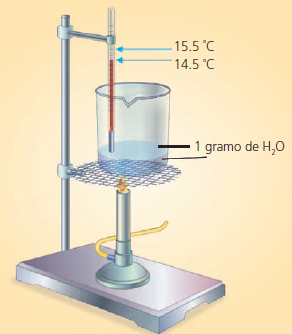
\includegraphics[scale=0.7]{Imagenes/Calor_04.png}
\end{figure}
\end{frame}
\begin{frame}
\frametitle{Ejercicio a cuenta}
Completa la siguiente tabla de conversión de unidades de calor.
\\
\bigskip
\pause
Deberás de incluir las correspondientes operaciones.
\end{frame}
\begin{frame}
\frametitle{Ejercicio a cuenta}
\begin{table}[H]
\small
\centering
\begin{tabular}{| c | c | c | c |} \hline
\unit{\joule} & \unit{\cal} & \unit{\kilo\cal} & \unit{\erg} \\ \hline
 & $100$ & & \\ \hline
 &  & $200$ & \\ \hline
 $500$ &  &  & \\ \hline
  &  &  & \num{2.5d8} \\ \hline
\end{tabular}
\end{table}
\end{frame}

\section{Transferencia de calor}
\frame{\tableofcontents[currentsection, hideothersubsections]}
\subsection{Tipos de transferencia}

\begin{frame}
\frametitle{Conducción}
Es el proceso mediante el cual el calor \textocolor{cadmiumgreen}{se transfiere directamente} a través de un material, \pause sin ningún
movimiento neto del material.
\end{frame}
\begin{frame}
\frametitle{Conducción}    
Por ejemplo, si acercas una varilla de metal a una flama, el calor que la flama emite se conduce al metal y éste a tu mano.
\end{frame}
\begin{frame}
\frametitle{Conducción}
\begin{figure}
    \centering
    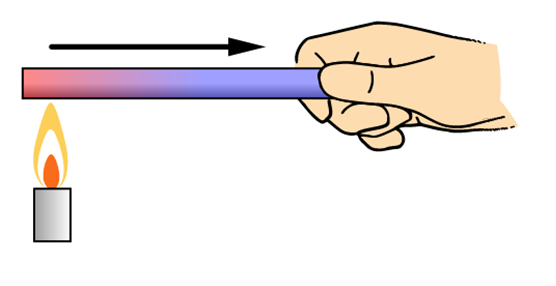
\includegraphics[scale=0.5]{Imagenes/Calor_03.png}
\end{figure}
\end{frame}
\begin{frame}
\frametitle{Radiación}
Es el proceso por el que los cuerpos \textocolor{cadmiumred}{emiten energía} que puede propagarse por el vacío.
\\
\bigskip
\pause
La energía radiante se transporta mediante ondas electromagnéticas.
\end{frame}
\begin{frame}
\frametitle{Radiación}
Por ejemplo, por la radiación nos llega el calor del sol, así como también por la radiación podemos sentir el
calor que se desprende de un foco encendido si acercamos la mano.
\end{frame}
\begin{frame}
\frametitle{Radiación}
\begin{figure}
    \centering
    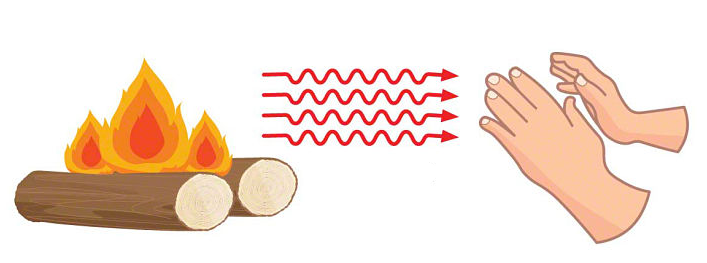
\includegraphics[scale=0.5]{Imagenes/Calor_02.png}
\end{figure}
\end{frame}
\begin{frame}
\frametitle{Convección}
Es el proceso por el cual el calor \textocolor{carmine}{se transfiere a través de un fluido} por el movimiento del mismo.
\end{frame}
\begin{frame}
\frametitle{Convección}
Por ejemplo, cuando se pone a calentar un recipiente con agua, ésta al calentarse en la parte inferior se dilata y disminuye su densidad.
\end{frame}
\begin{frame}
\frametitle{Convección}
\begin{figure}
    \centering
    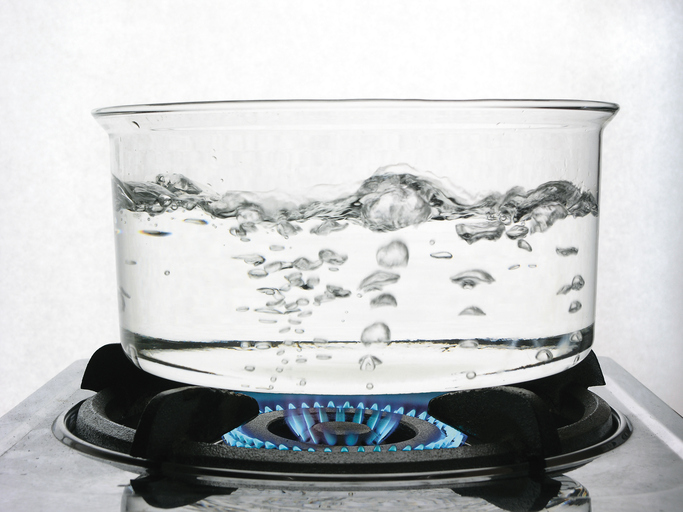
\includegraphics[scale=0.25]{Imagenes/Calor_01.jpg}
\end{figure}
\end{frame}
\begin{frame}
\frametitle{Convección}
Por lo que el agua caliente asciende y transporta así el calor de la parte inferior a la parte superior, generando un movimiento interno de las partículas.
\end{frame}

\section{Dilatación térmica}
\frame[allowframebreaks]{\tableofcontents[currentsection, hideothersubsections]}
\subsection{Definición}

\begin{frame}
\frametitle{¿Por qué se dilatan los cuerpos?}
La mayoría de los materiales se \textocolor{ao}{expanden} cuando su temperatura aumenta, \pause y se \textocolor{byzantine}{contraen} cuando la temperatura disminuye.
\end{frame}
\begin{frame}
\frametitle{¿Por qué se dilatan los cuerpos?}    
Esto ocurre porque al calentarse las moléculas se mueven más rápido y ocupan mayor espacio y esto hace que el cuerpo se expanda, \pause y cuando se enfría, las moléculas se mueven más lento y los materiales se contraen.
\end{frame}
\begin{frame}
\frametitle{¿Qué es la dilatación?}    
Este fenómeno se conoce como \textocolor{awesome}{dilatación}, \pause está estrechamente relacionado con los cambios de temperatura de los cuerpos.
\end{frame}
\begin{frame}
\frametitle{Ejemplos de dilatación térmica}
\begin{figure}
    \centering
    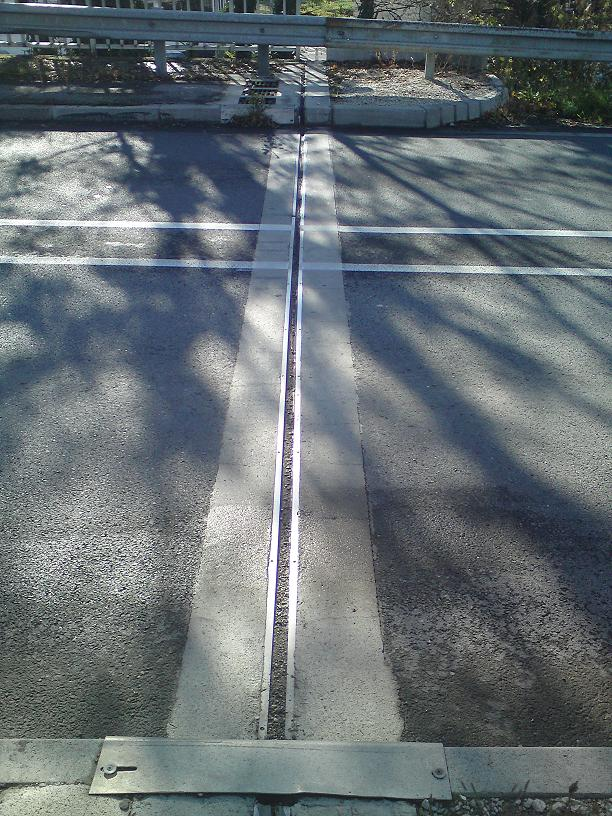
\includegraphics[scale=0.3]{Imagenes/Dilatacion_01.jpg}
\end{figure}
\end{frame}
\begin{frame}
\frametitle{Ejemplos de dilatación térmica}
\begin{figure}
    \centering
    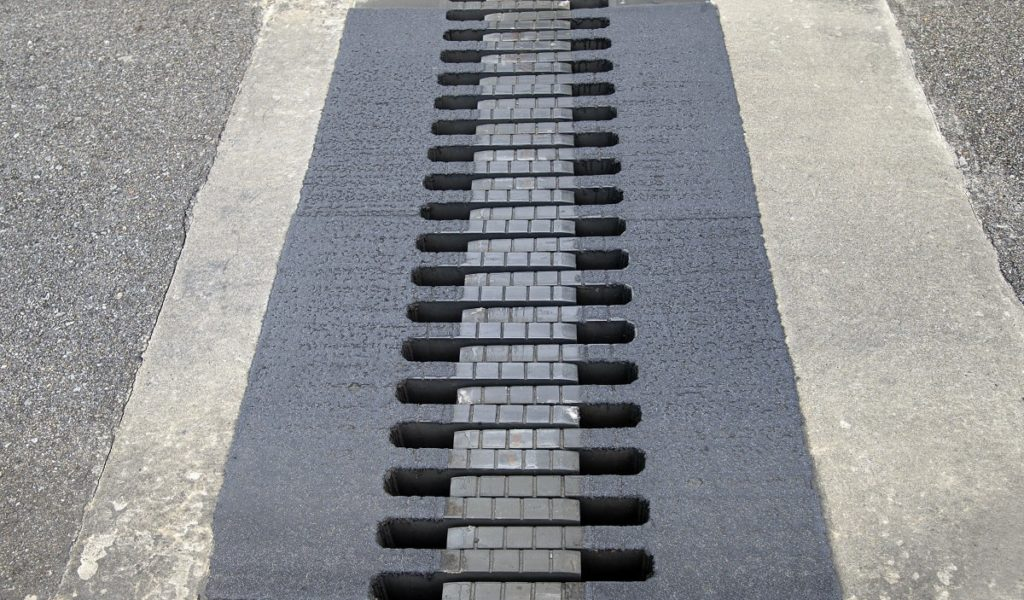
\includegraphics[scale=0.3]{Imagenes/Dilatacion_02.jpg}
\end{figure}
\end{frame}
\begin{frame}
\frametitle{Definición de dilatación}
La \textocolor{bulgarianrose}{dilatación térmica} es el aumento en sus dimensiones que experimenta un cuerpo cuando aumenta la temperatura, permaneciendo la presión constante.
\end{frame}
\begin{frame}
\frametitle{Tipos de dilatación}
Los sólidos se dilatan aumentando su \textocolor{carnelian}{longitud} principalmente, \pause aunque también pueden dilatarse en su \textocolor{coquelicot}{superficie} \pause o \textocolor{cordovan}{volumen}.
\end{frame}
\begin{frame}
\frametitle{Tipos de dilatación}
Al igual que los sólidos, los líquidos y los gases también aumentan o disminuyen su volumen, sin embargo, los gases se dilatan más que los líquidos.
\end{frame}

\subsection{Dilatación lineal}

\begin{frame}
\frametitle{Describiendo la dilatación lineal}
Se ha comprobado experimentalmente que al aumentar la temperatura de una barra, aumenta su \textocolor{cornellred}{longitud} \pause y este aumento es proporcional a su \textocolor{darkcyan}{longitud inicial} \pause y al \textocolor{darkscarlet}{aumento de su temperatura}.
\end{frame}
\begin{frame}
\frametitle{Describiendo la dilatación lineal}
A dicho proceso se le conoce como \textocolor{debianred}{dilatación lineal} y se expresa matemáticamente de la siguiente manera:
\pause
\begin{align*}
\Delta L = \alpha \, L_{i} \, \Delta T
\end{align*}
\end{frame}
\begin{frame}
\frametitle{La dilatación lineal}
\vspace*{-1cm}
\begin{align*}
\Delta L = \alpha \, L_{i} \, \Delta T
\end{align*}
Donde:
\setbeamercolor{item projected}{bg=deeppeach,fg=black}
\setbeamertemplate{enumerate items}{%
\usebeamercolor[bg]{item projected}%
\raisebox{1.5pt}{\colorbox{bg}{\color{fg}\footnotesize\insertenumlabel}}%
}
\begin{enumerate}[<+->]
\item $\Delta L$ es la variación de longitud.
\item $\alpha$ es el coeficiente de proporcionalidad, llamado \textocolor{denim}{coeficiente de dilatación lineal}, es un valor específico para cada material o sustancia.
\seti
\end{enumerate}
\end{frame}
\begin{frame}
\frametitle{Algunos coeficientes}
\begin{table}
    \centering
    \small
    \begin{tabular}{| l | c |} \hline
        Material & $\alpha \, (\unit{\degreeCelsius}^{-1})$ \\ \hline
        Concreto & $\numrange{0.7}{1.2d-5}$ \\ \hline
        Plata & \num{2.0d-5} \\ \hline
        Oro & \num{1.5d-5} \\ \hline
        Cobre & \num{1.7d-5} \\ \hline
    \end{tabular}
\end{table}
\end{frame}
\begin{frame}
\frametitle{Ejercicio Evaluación Continua}
Completa la siguiente tabla con los coeficientes de dilatación térmica:
\pause

Zinc, Vidrio Pirex, Aluminio, Acetona, Mercurio, Gasolina, Petróleo, Agua a \SI{100}{\degreeCelsius}, Aire, Latón.
\end{frame}
\begin{frame}
\frametitle{La dilatación lineal}
\vspace*{-1cm}
\begin{align*}
\Delta L = \alpha \, L_{i} \, \Delta T
\end{align*}
Donde:
\setbeamercolor{item projected}{bg=deeppeach,fg=black}
\setbeamertemplate{enumerate items}{%
\usebeamercolor[bg]{item projected}%
\raisebox{1.5pt}{\colorbox{bg}{\color{fg}\footnotesize\insertenumlabel}}%
}
\begin{enumerate}[<+->]
\conti
\item $L_{i}$ es la longitud inicial.
\item $\Delta T$ es la variación de la temperatura.
\end{enumerate}
\end{frame}
\begin{frame}
\frametitle{Consideraciones}
La variación de la longitud $\Delta L$ es la diferencia entre la longitud final, $L_{f}$ y la longitud inicial, $L_{i}$:
\pause
\begin{align*}
\Delta L = L_{f} - L_{i}
\end{align*}
\end{frame}
\begin{frame}
\frametitle{Consideraciones}
La variación de la temperatura $\Delta T$ es la diferencia entre la temperatura final, $T_{f}$ y la temperatura inicial, $T_{i}$:
\pause
\begin{align*}
\Delta T = T_{f} - T_{i}
\end{align*}
\end{frame}
\begin{frame}
\frametitle{La dilatación lineal}
La expresión para la dilatación lineal la podemos expresar como:
\pause
\begin{align*}
L_{f} - L_{i} = \alpha \, L_{i} \, \left( T_{f} - T_{i} \right)
\end{align*}
Expresión que nos será de mucha utilidad.
\end{frame}
\begin{frame}
\frametitle{Calculando el coeficiente de dilatación}
Ya que si nos proporcionan la longitud inicial, la final, así como el incremento de la temperatura, podemos calcular el coeficiente de dilatación:
\end{frame}
\begin{frame}
\frametitle{Calculando el coeficiente de dilatación}
Tenemos que:
\pause
\begin{eqnarray*}
\begin{aligned}
L_{f} - L_{i} &= \alpha \, L_{i} \, \left( T_{f} - T_{i} \right) \\[0.5em] \pause
\alpha &= \dfrac{L_{f} - L_{i}}{L_{i} \, \left( T_{f} - T_{i} \right)}
\end{aligned}
\end{eqnarray*}
\end{frame}
\begin{frame}
\frametitle{El álgebra en la expresión}
Si nos dan el valor de $\alpha$ y nos piden calcular la longitud final, hacemos el manejo algebraico de la expresión:
\pause
\begin{eqnarray*}
\begin{aligned}
L_{f} - L_{i} &= \alpha \, L_{i} \, \left( T_{f} - T_{i} \right) \\[0.5em] \pause
L_{f} &= \bigg[ \alpha \, L_{i} \, \left( T_{f} - T_{i} \right) \bigg] + L_{i} \\[0.5em] \pause
L_{f} &= L_{i} \bigg[ 1 + \alpha \, \left( T_{f} - T_{i} \right) \bigg]
\end{aligned}
\end{eqnarray*}
\end{frame}
\begin{frame}
\frametitle{Ejercicio 1 - Dilatación lineal}
A una temperatura de \SI{15}{\degreeCelsius} una varilla de hierro tiene una longitud de \SI{5}{\meter}
\\
\bigskip
\pause 
¿Cuál será la longitud al aumentar la temperatura a \SI{25}{\degreeCelsius}?
\end{frame}
\begin{frame}
\frametitle{Resolviendo el ejercicio}
\textocolor{red}{Datos:}
\begin{align*}
\alpha_{Fe} &= \num{11.7d-6} \unit{\degreeCelsius}^{-1} \\
L_{i} &= \SI{5}{\meter} \\
T_{i} &= \SI{15}{\degreeCelsius} \\
T_{f} &= \SI{25}{\degreeCelsius} \\
L_{f} &= \,?
\end{align*}
\end{frame}
\begin{frame}
\frametitle{Resolviendo el ejercicio}
\textocolor{red}{Expresión:}
\begin{align*}
L_{f} &= L_{i} \bigg[ 1 + \alpha \, \left( T_{f} - T_{i} \right) \bigg]
\end{align*}
\end{frame}
\begin{frame}
\frametitle{Resolviendo el ejercicio}
\textocolor{red}{Sustitución:}
\begin{eqnarray*}
\begin{aligned}
L_{f} &= \SI{5}{\meter} \bigg[ 1 + \num{11.7d-6} \unit{\degreeCelsius}^{-1} \, \left( \SI{25}{\degreeCelsius} - \SI{15}{\degreeCelsius} \right) \bigg] = \\[0.5em] \pause
L_{f} &= \SI{5.000585}{\meter}
\end{aligned}
\end{eqnarray*}
\end{frame}
\begin{frame}
\frametitle{Dilatación en la varilla}
Ahora ya podemos calcular la dilatación en la varilla:
\pause
\begin{eqnarray*}
\begin{aligned}
L_{f} - L_{i} &= \SI{5.000585}{\meter} - \SI{5}{\meter} = \\[0.5em] \pause
&= \SI{5.85d-4}{\meter}
\end{aligned}
\end{eqnarray*}
\end{frame}
    
\end{document}